\subsection{Measure}

Measure and integration theory develops the necessary tool for solving PDEs and stochastic processes.

\paragraph{$\sigma$-Algebra}

\subparagraph{Motivation}

In physics, the task of finiding ``volume'' is ubquitous. For instance in computing mass, charge, the integral would resemble:
\begin{equation}
\int (\cdot ) dV
\end{equation}
In some sense, this $dV$ is a function $dV:E\to \mathbb{R}$ which computes the volume of $E\subset \mathbb{R}^n$, a tiny control volume we are interested in.  It would be very natural to ask for this function to satisfy:

\begin{mystthmdefinition}{Measure}{definition-measure-1}Suppose $X$ is a set. Let $\mu: A \to \mathbb{R}$ where $A\in P(X)$ such that:

\begin{itemize}
\item \begin{equation}
\mu(\varnothing)=0
\end{equation}


\item \textbf{(countable additivity)} $E_1,E_2,....$ is a countable inifnite sequence of disjoint, then:

\begin{equation}
\mu(\cup_j E_j)=\sum_j \mu(E_j)
\end{equation}


Then we call $\mu$ a measure.
\end{itemize}

\end{mystthmdefinition}
The question would be, when can we find such a function. Trivially we can obtain such property by sending every $A$ to 0. However, for more practical purposes of modeling the world, we would like nicer properties. In particular, let's consider this compeletly reasonable demand on $\mathbb{R}^n$.

\begin{mystexercise}{Open Set as a Topology}{open_set_as_a_topology}\label{open_set_as_a_topology}\begin{enumerate}
\item Let $\mathcal{B}$ be the family of all open intervals in $\mathbb{R}$, i.e. subsets of the form
\begin{equation}
(a, b) := \{c \in \mathbb{R} \mid a < c < b\}
\end{equation}
for all $a, b \in \mathbb{R}$ with $a < b$. Let $\mathcal{T}(\mathcal{B})$ be the family of all arbitrary unions of elements in $\mathcal{B}$, i.e.,
\begin{equation}
\mathcal{T}(\mathcal{B}) := \left\{ \bigcup_{B \in \mathcal{B}'} B \mathrel{\Big\vert{}} \mathcal{B}' \subseteq \mathcal{B} \right\}
\end{equation}
Prove that $\mathcal{T}(\mathcal{B})$ is a topology on $\mathbb{R}$. (This ``$\mathcal{B}$'' stands for a ``base'' = ``basis'' of a topology.)


\item For $\mathcal{B}$ and $\mathcal{T}(\mathcal{B})$ as above and any $U \in \mathcal{T}(\mathcal{B})$ (i.e., any open set), prove that there exists a countable family $\mathcal{B}'' \subseteq \mathcal{B}$ (of open intervals) such that $U = \bigcup_{B \in \mathcal{B}''} B$. (Hint: it might help to prove first that the union of any family of open intervals containing a given $x \in \mathbb{R}$ is a generalized open interval in the sense that it is of the form $(a, b)$, $( -\infty, a)$ or $(a, \infty)$ for some $a, b \in \mathbb{R}$. Or do this any other way.)
\item For $\mathcal{T}(\mathcal{B})$ as above, prove that $\mathcal{T}(\mathcal{B}) \subseteq \mathcal{B}_{\mathbb{R}}$, the Borel $\sigma$-algebra on $\mathbb{R}$. (This ``$\mathcal{B}$'', confusingly, stands for ``Borel''.)
\item Use the above to give a full proof of Proposition 1.2 on p. 22 in [F].
\item Also deduce that $\mathcal{M}(\mathcal{B}) = \mathcal{M}(\mathcal{T}(\mathcal{B})) = \mathcal{B}_{\mathbb{R}}$.
\end{enumerate}

\end{mystexercise}
\begin{mystsolution}{Solution to Exercise~\ref{open_set_as_a_topology}}\begin{enumerate}
\item We prove that $\mathcal{T}(\mathcal{B})$ is a topology on $\mathbb{R}$.
\end{enumerate}

\begin{itemize}
\item \textbf{Property 1: $\emptyset, \mathbb{R} \in \mathcal{T}(\mathcal{B})$}

\begin{itemize}
\item $\emptyset = \cup_{B \in \emptyset} B$ (empty union), so $\emptyset \in \mathcal{T}(\mathcal{B})$
\item $\mathbb{R} = ( -\infty, \infty)$ is a generalized open interval, hence $\mathbb{R} \in \mathcal{T}(\mathcal{B})$. More explicitly, we can cover it by $\cup_{a=0}^{\infty} \{(a,a+1),( -a -1, -a)\}$
\end{itemize}


\item \textbf{Property 2: Closed under arbitrary unions}

\begin{itemize}
\item Let $\mathcal{U} \subseteq \mathcal{T}(\mathcal{B})$ be an arbitrary collection of sets in $\mathcal{T}(\mathcal{B})$. For each $U \in \mathcal{U}$, we have $U = \cup_{B \in \mathcal{B}_U} B$ for some $\mathcal{B}_U \subseteq \mathcal{B}$. Then $\cup_{U \in \mathcal{U}} U = \cup_{U \in \mathcal{U}} \left(\cup_{B \in \mathcal{B}_U} B\right) = \cup_{B \in \cup_{U \in \mathcal{U}} \mathcal{B}_U} B$. Since $\cup_{U \in \mathcal{U}} \mathcal{B}_U \subseteq \mathcal{B}$, we have $\cup_{U \in \mathcal{U}} U \in \mathcal{T}(\mathcal{B})$
\end{itemize}


\item \textbf{Property 3: Closed under finite intersections}

\begin{itemize}
\item By induction on the number $n$ of sets.
\item \textbf{Base case} ($n=1$): Trivial, $U \in \mathcal{T}(\mathcal{B})$.
\item \textbf{Inductive step}: Assume $U_1 \cap \cdots \cap U_n \in \mathcal{T}(\mathcal{B})$ for any $n$ sets in $\mathcal{T}(\mathcal{B})$.
For $n+1$ sets, write $(U_1 \cap \cdots \cap U_n) \cap U_{n+1}$. By induction hypothesis, $U_1 \cap \cdots \cap U_n = \cup_{i \in I}(a_i, b_i)$
for some countable collection of open intervals. Then

\begin{equation}
(U_1 \cap \cdots \cap U_n) \cap U_{n+1} = \left(\cup_{i \in I}(a_i, b_i)\right) \cap U_{n+1} = \cup_{i \in I}((a_i, b_i) \cap U_{n+1})
\end{equation}


Each $(a_i, b_i) \cap U_{n+1}$ is an intersection of an open interval with a union of open intervals, which is
a finite union of open intervals (or empty). Hence $(U_1 \cap \cdots \cap U_{n+1}) \in \mathcal{T}(\mathcal{B})$.
\end{itemize}
\end{itemize}

Therefore $\mathcal{T}(\mathcal{B})$ is a topology on $\mathbb{R}$.


\bigskip
\centerline{\rule{13cm}{0.4pt}}
\bigskip

\begin{enumerate}[resume]
\item Suppose $\mathcal B' \subseteq \mathcal B$ and

\begin{equation}
U=\bigcup_{B\in \mathcal B'} B
\end{equation}


where $\mathcal B'$ can be uncountable. We would like to show $\exists \mathcal B''$ that is countable such that

\begin{equation}
U=\bigcup_{B\in \mathcal B^{''}} B
\end{equation}


We now show a specfic way to construct $\mathcal B''$ from $\mathcal B'$. Define:

\begin{equation}
\mathcal B_x = \{(a,b)\in \mathcal B' : x\in (a,b)\}
\end{equation}


Clearly $\mathcal B_x \subseteq \mathcal B'$. Now proceed with the following procedure(an ``infinite algorithm'')on the construction of $\mathcal B''$
\end{enumerate}

\begin{mystthmalgorithm}{}{algorithm-measure-2}\textbf{Input}: A potentially uncountable set of open intervals $\mathcal B'$ such that $\cup \mathcal B'=U$

\textbf{Output}: A countable set of open intervals $\mathcal B''$ such that $\cup \mathcal B''=U$

\begin{enumerate}
\item $\mathcal B'' = \varnothing$
\item \textbf{While} $\exists x\in U$,  $x\notin \cup \mathcal B''$ :

\begin{enumerate}
\item Compute $(c,d)=\bigcup_{B\in \mathcal B_x} B$ where $c,d$ is in extended real number system.
\item \textbf{If} $c,d\in \mathbb{R}$:

\begin{enumerate}
\item $\mathcal{B}_x'=\{(c,d)\}$
\end{enumerate}


\item \textbf{Else if} $c\in \mathbb{R}, d=\infty$:

\begin{enumerate}
\item $\mathcal{B}_x'\gets \{(c,[c])\}\cup \{[c],[c]+j\}_{j=1}^{\infty}$
\end{enumerate}


\item \textbf{Else}
Other cases follows as (3)
\item $\mathcal B'' = \mathcal B'' \cup \mathcal B_x '$
\end{enumerate}


\item \textbf{Return} $\mathcal B''$
\end{enumerate}

\end{mystthmalgorithm}
where $[c]$ picks the closes integer towards the right of the real axis.
Note we implicitly invoked the claim below in computing $(c,d)$:

\begin{itemize}
\item $\boxed{\textbf{Cliam 1}}$ The union of arbitrary family of open intervals containing $x\in \mathbb{R}$ is a \textit{generalized open interval}

\begin{equation}
\bigcup_{B\in \mathcal B_x} B\in \{(c,d): c,d\in \mathbb{R}\cup \{\infty, -\infty\}\}
\end{equation}

\begin{itemize}
\item I claim the union is just $(c,d)$ where $c=\inf \{a:(a,b)\in \mathcal B_x\}$ and $d=\sup \{b:(a,b)\in \mathcal B_x\}$ where we allow $\infty$ and $-\infty$. Clearly $(c,d)$ covers $\cup \mathcal B_x$. It suffice to show $\cup \mathcal B_x$ covers $(c,d)$. Suppose $\exists y \in (c,d)$ and $y\notin \cup \mathcal B_x$. This means $\cup \mathcal B_x$ has a hole and there must exists a pair of open interval in $\mathcal B_x$ that is disjoint, contradicting that all open intervals in $\mathcal B_x$ contains $x$(in that case no pair should be disjoint).
\end{itemize}
\end{itemize}

Now what's left to show is (1) Only countable number of $\mathcal B_x'$ is needed. (2) each $\mathcal B_x'$ is countable. The later is obvious by construction. The former can be argued by countability of $\mathbb{Q}$. Pick a $q\in \mathbb{Q}$ in one of the open interval of $\mathcal B_x'$, this is always possible by density of rationals. Suppose uncountable $\mathcal B_x'$ is needed to cover $\cup \mathcal B''$ then $U=\cup \mathcal B''$ would contain uncountable number of rationals. This finishes the proof.


\bigskip
\centerline{\rule{13cm}{0.4pt}}
\bigskip

\begin{enumerate}[resume]
\item By definition, $\mathcal B_{\mathbb{R}}$ is the smallest $\sigma$-algebra containing $\mathcal T(\mathcal B)$. Therefore the inclusion holds by construction.
\end{enumerate}


\bigskip
\centerline{\rule{13cm}{0.4pt}}
\bigskip

\begin{enumerate}[resume]
\item We only need to show (b), (c), and (e) since (a) and (d) are generalized open
intervals and are actually shown by (5).
\end{enumerate}

\textbf{Case (b): Closed intervals} $\mathcal{E}_2 = \{[a,b]: a < b\}$

\begin{itemize}
\item $\mathcal{M}(\mathcal{E}_2) \subseteq \mathcal{B}_\mathbb{R}$: Note that $[a,b] = \cap_{j=1}^{\infty}(a -1/j, b+1/j)$
is a countable intersection of open intervals, so $\mathcal{E}_2 \subset \mathcal{B}_\mathbb{R}$.
\item $\mathcal{B}_\mathbb{R} \subseteq \mathcal{M}(\mathcal{E}_2)$: $(a,b) = \cup_{j=1}^{\infty}[a+1/j, b -1/j]$
is a countable union of closed intervals, so $\mathcal{B} \subset \mathcal{M}(\mathcal{E}_2)$ and hence
$\mathcal{B}_\mathbb{R} = \mathcal{M}(\mathcal{B}) \subset \mathcal{M}(\mathcal{E}_2)$.
\end{itemize}

\textbf{Case (c): Half-open intervals} $\mathcal{E}_3 = \{(a,b]: a < b\}$

\begin{itemize}
\item $\mathcal{M}(\mathcal{E}_3) \subseteq \mathcal{B}_\mathbb{R}$: $(a,b] = (a,b) \cup \{b\}$ where $(a,b) \in \mathcal{B}_\mathbb{R}$
and $\{b\} = \cap_{j=1}^{\infty}(b -1/j, b+1/j) \in \mathcal{B}_\mathbb{R}$.
\item $\mathcal{B}_\mathbb{R} \subseteq \mathcal{M}(\mathcal{E}_3)$: $(a,b) = \cup_{j=1}^{\infty}(a, b -1/j]$
is a countable union of half-open intervals, so $\mathcal{B} \subset \mathcal{M}(\mathcal{E}_3)$ and hence
$\mathcal{B}_\mathbb{R} \subset \mathcal{M}(\mathcal{E}_3)$.
\end{itemize}

\textbf{Case (e): Closed rays} $\mathcal{E}_7 = \{[a,\infty): a \in \mathbb{R}\}$

\begin{itemize}
\item $\mathcal{M}(\mathcal{E}_7) \subseteq \mathcal{B}_\mathbb{R}$: $[a,\infty) = \cap_{j=1}^{\infty}(a -1/j, \infty)$
is a countable intersection of open rays (generalized open intervals), so $\mathcal{E}_7 \subset \mathcal{B}_\mathbb{R}$.
\item $\mathcal{B}_\mathbb{R} \subseteq \mathcal{M}(\mathcal{E}_7)$: $(a,b) = (a,\infty) \cap ( -\infty,b)$ where
$(a,\infty) = \cup_{j=1}^{\infty}[a+1/j,\infty)$ and $( -\infty,b) = \mathbb{R} \setminus [b,\infty)$ are in $\mathcal{M}(\mathcal{E}_7)$,
so $\mathcal{B} \subset \mathcal{M}(\mathcal{E}_7)$ and hence $\mathcal{B}_\mathbb{R} \subset \mathcal{M}(\mathcal{E}_7)$.
\end{itemize}

Cases (c'), (e') follow by symmetry.


\bigskip
\centerline{\rule{13cm}{0.4pt}}
\bigskip

\begin{enumerate}[resume]
\item We only need to show

\begin{equation}
\begin{aligned}
\mathcal B &\subseteq \mathcal M(\mathcal T(\mathcal B)) \\
\mathcal T(\mathcal B) &\subseteq \mathcal M( \mathcal B)
\end{aligned}
\end{equation}
\end{enumerate}

\begin{itemize}
\item The former is trivial since $\mathcal B \subseteq \mathcal T(\mathcal B)\subseteq \mathcal M(\mathcal T(\mathcal B)$
\item The later can be shown using (2). $\mathcal M(\mathcal B)$ contains all countable unions of open intervals $\mathcal B$ while $\mathcal T(\mathcal B)$ contains arbitrary union. (2) bridges the gap by claiming the arbitrary union can actually be replaced by countable union.
\end{itemize}

\end{mystsolution}
\subsubsection{Construction of Measure}

\paragraph{The big picture}

The general idea of constructing measure is, in crude terms:

\begin{enumerate}
\item Find a collection of set that has a clear notion of size
\item Approximate arbitrary subsets using element in the elementary set, hence get a notion of size on arbtirary subsets
\item Make the notion of size truely a measure by restricting to a special collection of subset.
\end{enumerate}

Observe how the notion of size ripens:
\begin{equation}
\label{workflow_from_elementary_set}
\begin{aligned}
\text{Stage 1: $\boxed{|\cdot|:\mathcal E \to \mathbb{R}^+}$} 
&\longrightarrow \text{Stage 2: $\boxed{\mu^* : P(X)\to \mathbb{R}^+}$} \\ 
&\longrightarrow \text{Stage 3: $\boxed{\mu: \mathcal M|_{\mu^*} \to \mathbb{R}^{+}}$}
\end{aligned}
\end{equation}
\begin{enumerate}
\item \textit{Stage 1 to 2}: Create a notion of size on arbitrary sets $A\subset P(X)$ by approximating them using ``building blocks''$(A\in \mathcal E)$ which has a notion of size $|\cdot |$. This scarifices additivity and we instead of countable sub-additivity
\item \textit{Stage 2 to 3}: Shrink the domain by restrict to a particular family $\mathcal M |_{\mu^*}\subset P(X)$. This gives us \textit{countable additivity} and $\mu$ is now a \textbf{complete measure}
\end{enumerate}

\begin{mystthmexample}{}{example-measure-3}Concretely, think $\mathcal E$ as the set of all open rectangles in $\mathbb{R}^2$:
\begin{equation}
\mathcal E= \{(a,b)\times (c,d) | a<b,c<d; a,b,c,d\in \mathbb{R}\}
\end{equation}
These clearly ``canonical'' notion of size, namingly:
\begin{equation}
|A|=(d-c)(b-a)
\end{equation}
Now using these as ``building blocks'', we can measure arbitrary sets $E\in P(\mathbb{R}^2)$, for instance, a unit circle.
Here is a quick numerical demo for approximating a unit circle denoted by $E$ with squares on a grid. The resolution $n$ is defined as the number of intervals in $(0,1)$.

As we take finer and finer squares, we approach a limit(or the liminf). This number can be used as a notion of size for the set $E$. This motivates the definition of \textit{outer measure}.

\begin{mystadmonition}{mystGreen}{How did we compute that?}A simple way is to count grid points that is inside the unit circle. A quick \texttt{julia} implementation gives the above plot:

\begin{mystcodebox}
\begin{verbatim}
function compute_area_of_circle(n)
    cover::Int = 0
    for i in -n:n
        for j in -n:n
            if ((i/n)^2 + (j/n)^2) < 1
                if i == 0 && j == 0
                    cover += 4
                elseif i == 0 || j == 0 
                    cover += 2
                else 
                    cover += 1
                end 
            end
        end
    end
    return cover * (1/n)^2
end
\end{verbatim}

\end{mystcodebox}

\end{mystadmonition}
\end{mystthmexample}
\begin{figure}[!htbp]
\centering
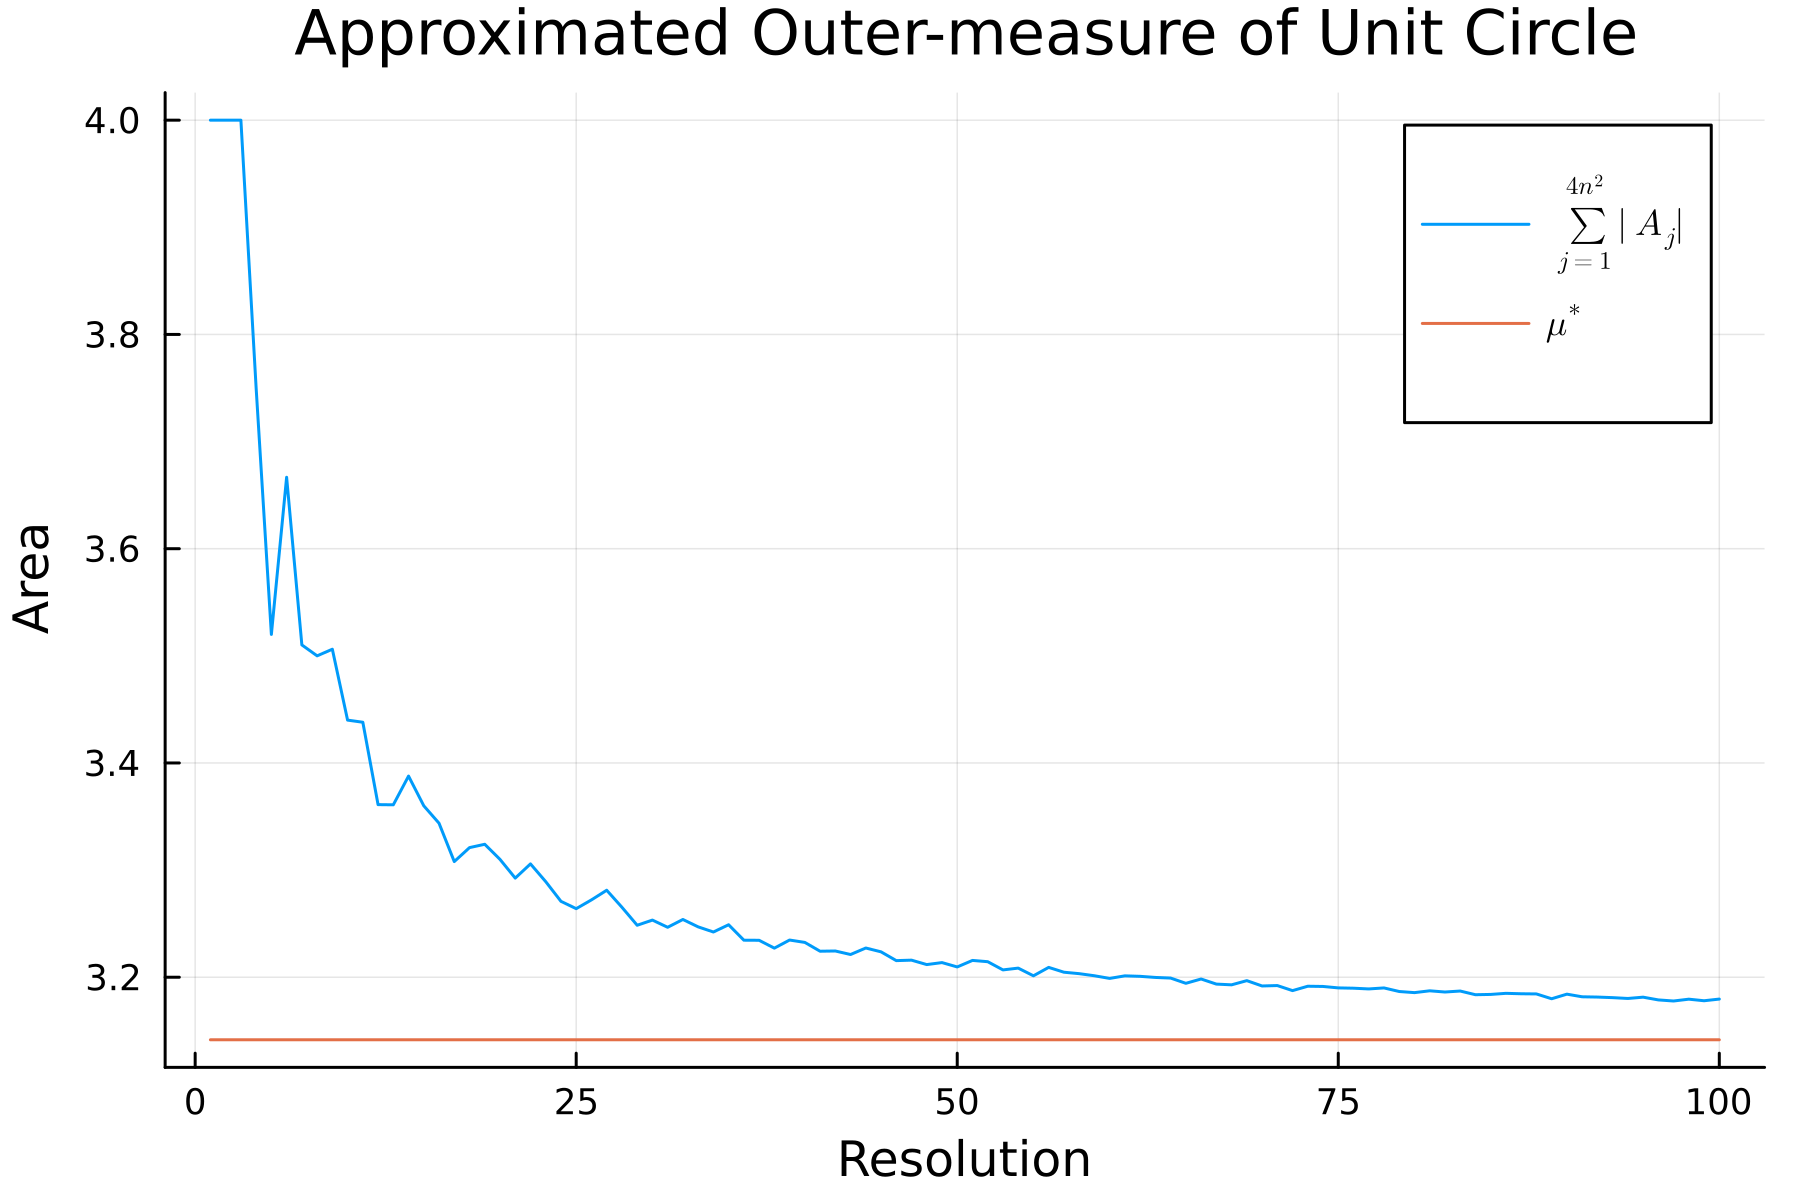
\includegraphics[width=0.7\linewidth]{files/outer_measure_of_uni-0984d03216df07ccde5cf8a5a0f6b7d4.png}
\end{figure}

\paragraph{Outer Measure}

So how do we actually construct measures no matter what set we are working on?(Though in this book we are really interested in just $\mathbb{R}^n$). A general guidline is:

\begin{enumerate}
\item Find some \textit{elementary set} $\mathcal{E}$ where premeasure is defined on the disjoint uniont of $\mathcal{E}$.
\item Define the measure of arbitrary subset $A\in P(X)$ as the the size of ``smallest'' cover of $A$ using the elementary set:
\end{enumerate}
\begin{equation}
\label{omfml}
\inf \left\{\sum_{\nu=1}^{\infty} \rho(E_{\nu}): E_{\nu}\in \mathcal{E}, A\subset \bigcup_{\nu=1}^{\infty} E_{\nu}\right\}
\end{equation}
More generally we can define an \textit{outer measure} as follows:

\begin{mystthmdefinition}{Outer Measure}{omdf}\label{omdf}An outer measure on an non-empty set $X$ is a function $\mu^* : P(X)\to [0,\infty]$ such that:

\begin{itemize}
\item $\mu^*(\varnothing)=0$
\item If $A\subset B$, then $\mu^*(A)<\mu^*(B)$
\item $\mu^*(\cup_{\nu}A_{\nu})\leq \sum_{\nu} \mu^* (A_{\nu })$
\end{itemize}

\end{mystthmdefinition}
We note that property (2),(3) are both derived properties of measure. So we can think the definition of outer measure as a relaxation of measure: take out countable additvity and adds back two derived property. In addition,  We note that (\ref{omfml}) obeys Definition~\ref{omdf}

\begin{mystadmonition}{mystAmber}{Exercise}Show that (\ref{omfml}) indeed defines an outer measure Definition~\ref{omdf}.

\end{mystadmonition}
\paragraph{Carathéodory Family $\mathcal M_{\mu^*}$}

How do we then obtain measure from outer measure? We note that what outer measure lacks is finite additivity, so we can further ask, is there a collection of subset $\mathcal {M}\subset P(X)$ such that $\mu^*$ is actually finitey additive? The answer is actually YES! However this seems rather arbitrary:
\begin{equation}
\mathcal M = \{A\subset X: \mu^*(F)=\mu^*(F-A)+\mu^*(A\cap F), \forall F \subset X\}
\end{equation}
We call elements of $\mathcal M$ \textbf{$\mu^*$-measureable}. In plain English, this saying $A$ can ``split measure'' arbitrary $F\subset X$ by measuring the intersection and the complement separetly and add them together.

\begin{mystthmtheorem}{Carathéodory's Theorem}{theorem-measure-4}If $\mu^*$ is an outer measure of $X$ then

\begin{enumerate}
\item the collection of \textbf{$\mu^*$-measureable} sets:

\begin{equation}
\mathcal M = \{A\subset X: \mu^*(F)=\mu^*(A^c \cap F)+\mu^*(A\cap F), \forall F \subset X\}
\end{equation}


is a $\sigma$-algebra.


\item $\mu^*|_{\mathcal M}$ is a \textbf{complete measure}
\end{enumerate}

\end{mystthmtheorem}
\paragraph{Premeasure and The Extension Theorem}

THe workflow (\ref{workflow_from_elementary_set}) is already very promising except one key issue:

\begin{mystadmonition}{mystAmber}{Carathéodary Family can be Small}What if $\mathcal M_{\mu^*}$ is trivial or very samll?

\end{mystadmonition}
The next theorem prevents this by starting with an \textit{algebra} $\mathcal A$ instead of just a plain family of sets $\mathcal E$.  The plain notion of size on $\mathcal E$ is replaced by the so-called \textit{premeasure}.

\begin{mystthmdefinition}{Premeasure}{definition-measure-5}Suppose $\mathcal A\subset \mathcal P(X)$ is an algebra, a function $\mu_0 : \mathcal A\to [0,\infty]$ is a \textbf{premeasure} if

\begin{enumerate}
\item $\mu_0(\varnothing)=0$
\item Let $\{A_j\}_1^{\infty}$ is a sequence of disjoint sets in $\mathcal A$. Given $\bigcup_1^{\infty} A_j \in \mathcal A$ then

\begin{equation}
\mu_0 \left( \bigcup_1^{\infty}\right) = \sum_{1}^{\infty} \mu_0(A_j)
\end{equation}
\end{enumerate}

\end{mystthmdefinition}
\begin{mystexercise}{Completeness of $\mathcal M_{\mu^*}$}{completeness_of_mathcal_m_mu}\label{completeness_of_mathcal_m_mu}A measure $\mu$ on a $\sigma$-algebra $\mathcal{M}$ is complete if
\begin{equation}
\forall N \in \mathcal{M} \quad \forall N' \subseteq N \quad (\mu(N) = 0 \Rightarrow N' \in \mathcal{M}).
\end{equation}
Let $\mu^*$ be an outer measure on a set $X$. Prove that the measure on $\mathcal{M}_{\mu^*}$ induced by $\mu^*$ by the Carathéodory construction is complete. (The proof of Carathéodory theorem in the book does not explain this well, write a detailed proof.)

\end{mystexercise}
\begin{mystsolution}{Solution to Exercise~\ref{completeness_of_mathcal_m_mu}}\begin{mystthmproof}{}{proof-measure-6}Note that $\mu(N)=0\Longrightarrow \mu(N')=0$. $\forall E\subseteq X$, by subadditivity:
\begin{equation}
\mu^*(E) \leq \mu^*(E\cap N') + \mu^*(E\cap N'^c)
\end{equation}
By monotoncity and positivity of $\mu^*$ we have $\mu^*(E\cap N')=0$(since $E\cap N' \subseteq N'$ so $\mu^*(E\cap N')\leq 0$). But again by monotonicity $\mu^*(E\cap N'^c) \leq \mu^*(E)$ hence we have:
\begin{equation}
\mu^*(E) \leq \mu^*(E\cap N') + \mu^*(E\cap N'^c) \leq \mu^*(E)
\end{equation}
Hence:
\begin{equation}
\mu^*(E) = \mu^*(E\cap N') + \mu^*(E\cap N'^c)
\end{equation}
As desired.

\end{mystthmproof}
\end{mystsolution}
\begin{mystexercise}{}{folland_problem_18}\label{folland_problem_18}Let $\mathcal{A} \subset \mathcal{P}(X)$ be an algebra, $\mathcal{A}_\sigma$ the collection of countable unions of sets in $\mathcal{A}$, and $\mathcal{A}_{\sigma\delta}$ the collection of countable intersections of sets in $\mathcal{A}_\sigma$. Let $\mu_0$ be a premeasure on $\mathcal{A}$ and $\mu^*$ the induced outer measure.

\begin{enumerate}
\item For any $E \subset X$ and $\epsilon > 0$ there exists $A \in \mathcal{A}_\sigma$ with $E \subset A$ and $\mu^*(A) \le \mu^*(E) + \epsilon$.
\item If $\mu^*(E) < \infty$, then $E$ is $\mu^*$-measurable iff there exists $B \in \mathcal{A}_{\sigma\delta}$ with $E \subset B$ and $\mu^*(B \setminus E) = 0$.
\item If $\mu_0$ is $\sigma$-finite, the restriction $\mu^*(E) < \infty$ in (2) is superfluous.
\end{enumerate}

\end{mystexercise}
\begin{mystsolution}{Solution to Exercise~\ref{folland_problem_18}}1.This is just the definition of outer measure(namingly, infimum). Note since
\begin{equation}
\mu^*(E)= \inf C
\end{equation}
where
\begin{equation}
C= \left\{\sum \mu_0(A_j) | A=\cup A_j\in \mathcal A_{\sigma}, E\subset A \right\}
\end{equation}
Hence $\exists c\in C$ such that $c < \mu^*(E)+\epsilon$ by the definition of infimum. Now the map between open covers and their area is clearly surjective by construction:
\begin{equation}
\begin{aligned}
\{A\in \mathcal A_{\sigma} : E\subset A\} &\to \mathbb{R} \\
A &\mapsto \underbrace{\sum_j \mu_0(A_j)}_{\mu^*(A)}
\end{aligned}
\end{equation}
hence we can find $A\in A_{\sigma}$ that correponds to $c$.

\begin{enumerate}[resume]
\item $(\Longrightarrow)$ Suppose $E$ is $\mu^*$-measurable. Now by (1) we can find a sequence $\{A_n\}_{n=1}^{\infty}$ where $A_n\in \mathcal A_{\sigma}$, each covers $E$ and $\mu^*(A_n)\leq \mu^*(E)+\frac1n$.  By taking the intersection of the sequence and define that as $B$:

\begin{equation}
B:=\bigcap_{n}A_{n} \in A_{\sigma \delta}
\end{equation}


By construction $B$ covers $E$. Since $E\in \mathcal M_{\mu^*}$ where the later is an $\sigma$-algebra and $\mu^*$ is a complete measure on $\mathcal{M}_{\mu^*}$. We can use \textit{continuity-from-above} of outer-meassure if $\mu^*(E)<\infty$ that $\mu^*(A)=\lim_{n \to \infty}\mu^*(A_n)=\mu^*(E)$.
\end{enumerate}

$(\Longleftarrow)$ Suppose there exists $B\in \mathcal A_{\sigma \delta}$ such that $E\subset B$ and $\mu^*(B\setminus E)=0$. Note any $B\in \mathcal A_{\sigma \delta}$ is $\mu^*$-measurable since $\mathcal A \subset \mathcal M_{\mu^*}$(by \textit{extension theorem}).
We would like for all $F\subset X$
\begin{equation}
\mu^*(F) \geq  \mu^*(F\cap E) +\mu^*(F \cap E^c)
\end{equation}
But now $E\subset B$ hence:
\begin{equation}
\begin{aligned}
\mu^*(F) &= \mu^*(F\cap B) + \mu^*(F\cap B^c) \\ 
&\geq  \mu^*(F\cap E) + \mu^*(F\cap B^c)
\end{aligned}
\end{equation}
Note all we need now is $\mu^*(F \cap B^c) \geq  \mu^*(F\cap E^c)$.

But now
\begin{equation}
\mu^*(F\cap E^c) = \mu^*(F\cap (B^c \cup (B\cap E^c))) \leq \mu^*(F\cap B^c)  + \mu^*(F\cap (B\cap E^c))
\end{equation}

Again, by monotonicity and the assumption
\begin{equation}
\mu^*(F\cap (B\cap E^c))\leq \mu^*(B\cap E^c) = 0
\end{equation}
Therefore
$\mu^*(F \cap B^c) \geq  \mu^*(F\cap E^c)$. As desired.

\begin{enumerate}[resume]
\item Suppose $\mu_0$ is $\sigma$-finite then $\exists \{X_n\}$, $\mu_0(X_n)<\infty$ such that $X = \cup_n X_n$. Now define $E_n= X_n\cap E$, we can apply (2) to each $E_n$(There existss $B_n\in \mathcal A_{\sigma\delta}$ satisfying the property iff $E_n\in \mathcal M$).
\end{enumerate}

($\Longrightarrow$)  Say we already have desired set $B_n$ for each $E_n$. Take the union $B=\cup_n B_n$, now it satisfy the property since:
\begin{equation}
\begin{aligned}
\mu^*(B\setminus E) &=\mu^*(\bigcap_n (B_n \setminus E))  \\
&\leq \mu^*(B_1\setminus E) \\
&=1
\end{aligned}
\end{equation}
and it trivially covers $E$ since $E_n \subset B_n$.

($\Longleftarrow$) Suppose there is such $B$ for $E$(possibly infinite outer-measure) then we can construct $B_n$ and $E_n$ as before. Clearly each $B_n$ still satisfy the property hence we get $E_n \in \mathcal M$ by (2) since each $E_n$ has finite outer-measure. Now we want to show $E \in \mathcal M$ but this is trivial as $\sigma$-algebra is closed under union and $E= \cup E_n$

\end{mystsolution}
\begin{mystexercise}{}{folland_19}\label{folland_19}Let $\mu^*$ be an outer measure on $X$ induced from a finite premeasure $\mu_0$. If $E \subset X$, define the inner measure of $E$ to be $\mu_*(E) = \mu_0(X) - \mu^*(E^c)$. Then $E$ is $\mu^*$-measurable iff $\mu^*(E) = \mu_*(E)$

\end{mystexercise}
\begin{mystsolution}{Solution to Exercise~\ref{folland_19}}\end{mystsolution}
The following exercise is assumed everywhere in mathematics and is not directly related to outer measure. But they are invokded multiple times, for instance, in subadditivity of outer measure.

\begin{mystexercise}{Order invariance for Series of Positive Terms}{order_invariance_for_series_of_positive_terms}\label{order_invariance_for_series_of_positive_terms}\begin{enumerate}
\item Prove that any generalized series with summands in $[0, \infty]$ can be summed in any order. Specifically, if $a_j \in [0, \infty]$ for $j \in \mathbb{N} = \{1, 2, 3, \dots\}$, then for any bijection $\mathbb{N} \to \mathbb{N},\ j \mapsto k_j$, the equality $\sum_{j=1}^\infty a_j = \sum_{j=1}^\infty a_{k_j}$ holds. (That is, a nonnegative generalized series can be summed in any order.)
\item Prove that any two generalized series with summands in $[0, \infty]$ can be summed as one series. Specifically, if $a_j, b_j \in [0, \infty]$ for $j \in \mathbb{N}$, then the equality $\sum_{j=1}^\infty a_j + \sum_{j=1}^\infty b_j = \sum_{j=1}^\infty (a_j + b_j)$ holds.
\end{enumerate}

\end{mystexercise}
\begin{mystsolution}{Solution to Exercise~\ref{order_invariance_for_series_of_positive_terms}}\begin{enumerate}
\item We first make a claim

\begin{equation}
\sum_{j\in \mathbb{N}}a_j = \sup_J \sum_{j\in J} a_j
\end{equation}


where $J\subset \mathbb{N}, |J|<\infty$.
\end{enumerate}

\begin{itemize}
\item To show $\sum_{j\in \mathbb{N}} a_j  \leq \sup \sum_{j\in J} a_j$:
\begin{equation}
\sum_{j\in \mathbb{N}}a_j=\lim_{N\to\infty} \sum_{j=1}^N a_j \leq \sup \sum_{j\in J} a_j
\end{equation}


\item To show $\sum_{j\in \mathbb{N}} a_j  \geq \sup \sum_{j\in J} a_j$, we first note $\forall J$ as above:
\begin{equation}
\sum_{j\in \mathbb{N}} a_j = \sup_m s_m \geq s_{\max J} \geq  \sum_{j\in J} a_j
\end{equation}
Now $\sup$ perserves non-strict inequality so we can take $\sup$ on both sides to get:
\begin{equation}
\sup_{J} \sum_{j\in \mathbb{N}} a_j =  \sum_{j\in \mathbb{N}} a_j \geq  \sup_J \sum_{j\in J} a_j
\end{equation}
as desired.
Now (1) becomes trivial since $\forall J$ defined as above, suppose we define:
\begin{equation}
k(J)=\{k(j): j\in J\}
\end{equation}
now by the claim
\begin{equation}
\sum_{j\in \mathbb{N}} a_{k(j)} = \sup_{J} \sum_{j\in J'} a_j  = \sup_{J} \sum_{j\in k(J)} a_j
\end{equation}
where the last equality follows as $J'$ is also in the set $\{J\subset N: |J|<\infty\}$.
\end{itemize}


\bigskip
\centerline{\rule{13cm}{0.4pt}}
\bigskip

\begin{enumerate}
\item We first make a claim:
For monotone non-decreasing sequences $s_n, t_n$:

\begin{equation}
\sup(s_n + t_n) = \sup s_n + \sup t_n
\end{equation}
\end{enumerate}

\begin{itemize}
\item $\sup(s_n + t_n) \leq \sup s_n + \sup t_n$ is true since $\forall m, s_m + t_m \leq \sup s_n + \sup t_n$ and taking $\sup_m$ on both sides get us desired.
\item $\sup(s_n + t_n) \geq \sup s_n + \sup t_n$ can be shown by arguing $\forall \epsilon > 0$,

\begin{equation}
\sup(s_n + t_n) \geq \sup s_n + \sup t_n - \epsilon
\end{equation}


Deonte $s=\sup s_n, t = \sup t_n$. We can pick $N_1, N_2$ such that the corresponding tail follows $\sup s_n < s - \epsilon/2, \sup t_n < t - \epsilon /2$. Let $N=\max(N_1,N_2)$ then $\forall n > N$ we have:

\begin{equation}
\sup s_n + \sup t_n \leq  s + t - \epsilon
\end{equation}


As desired. (2) then easily follows by taking the claim in (1) and then let

\begin{equation}
\begin{aligned}
s_n &=\sum_{j=1}^n a_j \\
t_n &=\sum_{j=1}^m b_j
\end{aligned}
\end{equation}


Apply the above claim gets desired.
\end{itemize}

\end{mystsolution}
\subsubsection{Casestudy: Lebesgue-Stieltjes Measure}

The most useful set that we would like to equip a measure with is, unarguably, the real numbers $\mathbb{R}$.

\paragraph{Starting Point: The half-intervals}

Recall that we would start with an elementary collection that has a clear notion of size. We define the \textbf{h-intervals}:
\begin{equation}
H=\{(a,b]:a<b, a,b\in \mathbb{R}\}
\end{equation}

We define a terminology here:

\begin{mystthmdefinition}{Borel Sets}{definition-measure-7}Let $X$ any metric space, the $\sigma$-algebra genereated by the family of open sets in $X$ is called the \textbf{Borel $\sigma$-algebra}, denoted by $\mathcal B_{X}$

\end{mystthmdefinition}
\begin{mystexercise}{h-intervals generate $\mathcal B_{\mathbb{R}}$}{exercise-bg16v3fwbo}\label{exercise-bg16V3FwBo}\label{exercise-bg16v3fwbo}Check $H$ is an elementary set and so it generates an algebra $\mathcal A$. Furthermore, show that the $\sigma$-algebra generated by $\mathcal A$ is   $\mathcal B_{\mathbb{R}}$

\end{mystexercise}
Another terminology:

\begin{mystthmdefinition}{Elementary Decomposition}{definition-measure-8}Suppose $A\in \mathcal A$, since $\mathcal A=\mathcal M(H)$ we can find finite disjoint h-intervals $\{I_j\}_{j=1}^N=\{(a_j,b_j]_j\}_{j=1}^N$ such that:
\begin{equation}
A=\bigcup_{j=1}^N I_j
\end{equation}
Then $\{I_j\}$ is an \textbf{elementary decomposition} of $A$.

\end{mystthmdefinition}
We define size on $H$ as follows:

\begin{mystadmonition}{mystBlue}{Notion of Size on h-intervals}Let $F:\mathbb{R}\to\mathbb{R}$ be increasing and right-continous, let $(a,b]\in H$, then:
\begin{equation}
|(a,b]|=F(b)-F(a)
\end{equation}
Note when $F(x)=x$, we get the common notion of length of interval.

\end{mystadmonition}
The next step is to extend this notion of size to $\mathcal A=\mathcal M(H)$.

\paragraph{Step 1: Construction of a premeasure}

Now we have an algebra $\mathcal A$ where elements of the algebra $A\in \mathcal A$ has an elementary decomposition $A=\{I_j\}$ to h-intervals $I=(a_j,b_j]$, which is equipped with a notion of size $b_j -a_j$. A natural way to define the notion of size for $A$ is hence:
\begin{equation}
\mu_0(A) = \sum_{j=1}^N |I_j| =\sum_{j=1}^N F(b_j)-F(a_j)
\end{equation}
We claim that $\mu_0$ is actually a \textit{pre-measure} on $\mathcal A$.

\begin{mystthmproposition}{}{proposition-measure-9}Let $F:\mathbb{R}\to\mathbb{R}$ to be a right-continuous, increasing function. Define $\mu_0$ as
\begin{equation}
\begin{aligned}
\mu_0 : \mathcal A &\to \mathbb{R} \\
\bigcup_{j=1}^N A &\mapsto \sum_{j=1}^N [F(b_j)-F(a_j)]
\end{aligned}
\end{equation}
where $\{I_j\}=\{(a_j,b_j]\}$ is an elementary decomposition. Then $\mu_0$ is a premeasure on $\mathcal A$.

\end{mystthmproposition}
\begin{mystthmproof}{$\mu_0$ is a pre-measure}{proof-measure-10}We first need to show that $\mu_0$ is actually well-defined\footnote{Note that in definiting a notion of size $\mu_0$ on $A\in \mathcal A$, we requires $A$ to have a concrete representation $\cup_j I_j$. If the result is independent on
how we choose this representation(i.e. different elementary decomposition$\{I_j\}$), then this notion of size is indeed fundamentally correct. Otherwise if $\mu_0$ is dependent on how we choose representation, then it is not a credibe notion of size. Such ``representational invariance'' is called \textit{well-definedness} in mathematics.}. Then we illustrate:

\begin{enumerate}
\item Empty set has zero measure
\item Non-negativity
\item Finite additivity
\item Countable additivity
where only $(1),(2),(4)$ is truely required. But $(3)$ is used in the proof of $(4)$.
\end{enumerate}

\end{mystthmproof}